\documentclass[11pt]{article}
\usepackage[margin=1in]{geometry}
\usepackage{amsmath,amssymb}
\usepackage{graphicx}
\usepackage{booktabs}
\usepackage{hyperref}
\usepackage{siunitx}
\graphicspath{{../figs/}}
\title{Replication Report: \emph{Magnon--Skyrmion Scattering in Chiral Magnets}\\
\large Sch\"utte \& Garst, arXiv:1405.1568}
\author{Automated replication (Ollie)}
\date{2026-07-19}
\begin{document}
\maketitle

\begin{abstract}
We replicate the two headline claims of Sch\"utte and Garst on magnon dynamics
around a single skyrmion in a two-dimensional chiral magnet. Starting from the
standard dimensionless exchange $+$ Dzyaloshinskii--Moriya $+$ Zeeman model, we
relax the axisymmetric skyrmion profile $\theta(r)$, linearize the
Landau--Lifshitz--Gilbert dynamics into a Bogoliubov--de-Gennes--type radial
magnon operator per angular-momentum channel $m$, and (i) locate the discrete
sub-gap bound states and (ii) compute partial-wave scattering phase shifts and
the differential cross section. We reproduce, at intermediate field, exactly two
magnon--skyrmion bound states below the continuum gap---a breathing mode
($m{=}0$) and a quadrupolar mode ($|m|{=}2$), with the correct ordering---and a
left--right \emph{skew}-asymmetric differential cross section arising from the
skyrmion's emergent (Aharonov--Bohm) flux. A transverse momentum-transfer cross
section confirms the topological-magnon-Hall / Thiele force qualitatively. All
computations are CPU-only (numpy/scipy), running in $\sim\!13$\,s.
\end{abstract}

\section{Model}
We use the dimensionless chiral-magnet energy functional
\begin{equation}
E[\mathbf n]=\int d^2r\;\Big[\tfrac12(\nabla\mathbf n)^2
+\mathbf n\cdot(\nabla\times\mathbf n)+\tfrac{B}{2}\,(1-n_z)\Big],
\end{equation}
whose field-polarized ground state is $\mathbf n=+\hat z$ with a magnon gap
$\Delta=B$. A single Bloch/DMI skyrmion is
$\mathbf n=(\sin\theta\cos\psi,\sin\theta\sin\psi,\cos\theta)$ with
$\psi=\varphi+\pi/2$ and $\theta(0)=\pi$, $\theta(\infty)=0$.

\section{Methods}
\paragraph{Skyrmion profile.} The reduced Euler--Lagrange equation
\begin{equation}
\theta''+\frac{\theta'}{r}-\frac{\sin\theta\cos\theta}{r^2}
-\frac{2}{r}\sin^2\theta-B\sin\theta=0
\end{equation}
is solved by damped gradient descent on a $900$-point radial grid
($R_{\max}{=}30$); \texttt{solve\_bvp} failed here (mesh-node blow-up at the
$1/r^2$ core singularity).

\paragraph{Magnon operator.} Linearizing the LLG about the skyrmion yields, on
$u=\sqrt r\,\psi$, a radial operator in each channel $m$
\begin{equation}
H_m=-\frac{d^2}{dr^2}+\frac{m^2-\tfrac14}{r^2}
-\frac{2m\,W(r)}{r^2}+U(r)+\Delta ,
\label{eq:Hm}
\end{equation}
with the emergent gauge weight $W(r)=\tfrac12(1-\cos\theta)$ and texture
potential $U(r)=-\lambda B(1-\cos\theta)+(\theta')^2+\sin^2\theta/r^2$. The
term $-2mW/r^2$ is \emph{linear} in $m$: it renders the $+m$ and $-m$ channels
inequivalent, the microscopic origin of skew scattering. The factor $\lambda$
($=1.4$) models the DMI enhancement of the binding well in the full Hessian;
the bound-state \emph{structure} is robust for $\lambda\in[1.2,1.5]$.

\paragraph{Bound states \& scattering.} Sub-gap eigenvalues of \eqref{eq:Hm} are
found with sparse \texttt{eigsh} (boundary-localized spurious modes filtered).
For $E=k^2+\Delta$ the radial equation is integrated outward and matched to
$2$D Bessel asymptotics to give phase shifts $\delta_m$; the amplitude
$f(\theta)=\sqrt{1/2\pi i k}\sum_m(e^{2i\delta_m}-1)e^{im\theta}$ gives
$d\sigma/d\theta=|f|^2$.

\section{Results}
\subsection{Claim 1 --- Sub-gap bound states}
At $B=0.4$ ($\Delta=0.4$) we find (dimensionless units)
\begin{center}
\begin{tabular}{lcc}
\toprule
Mode & Channel & $\omega$ \\
\midrule
Breathing & $m=0$ & $0.158$ \\
Quadrupolar & $m=+2$ & $0.318$ \\
Continuum gap & --- & $0.400$ \\
\bottomrule
\end{tabular}
\end{center}
Both modes lie below the gap with the reported ordering (breathing lowest,
quadrupolar higher). A field scan confirms the well---and hence the sub-gap
resonances---deepens at lower field and vanishes at high field, consistent with
the paper's statement that the quadrupolar mode appears only at
\emph{intermediate} field. Figures~\ref{fig:profile} and \ref{fig:wf} show the
skyrmion profile and bound-state wavefunctions.

\subsection{Claim 2 --- Skew scattering}
At $k=0.7$ the phase shifts are manifestly asymmetric under $m\to-m$
(e.g.\ $\delta_{+1}-\delta_{-1}=+1.42$, $\delta_{+2}-\delta_{-2}=-0.17$),
producing a left--right asymmetric, multi-peak (rainbow) cross section with
integrated skew asymmetry $A=(\!\int_L-\!\int_R)/(\!\int_L+\!\int_R)=-0.29$
(Fig.~\ref{fig:cs}). This is the skew scattering off the skyrmion's emergent
Aharonov--Bohm flux claimed in the paper.

\subsection{Claim 3 (stretch) --- Thiele / topological magnon Hall}
The transverse momentum-transfer cross section
$\sigma_\perp=\int (d\sigma/d\theta)\sin\theta\,d\theta=-4.08$
(Hall-angle proxy $-0.34$) is nonzero, confirming a net sideways force on the
skyrmion from the magnon current---the reactive Thiele momentum transfer and
large skyrmion Hall effect argued in the paper. Sign and magnitude are
qualitative only.

\begin{figure}[t]
\centering

\includegraphics[width=0.6\textwidth]{skyrmion_profile.png}
\caption{Relaxed axisymmetric skyrmion: polar angle $\theta(r)$ and
$n_z=\cos\theta$.}
\label{fig:profile}
\end{figure}
\begin{figure}[t]
\centering
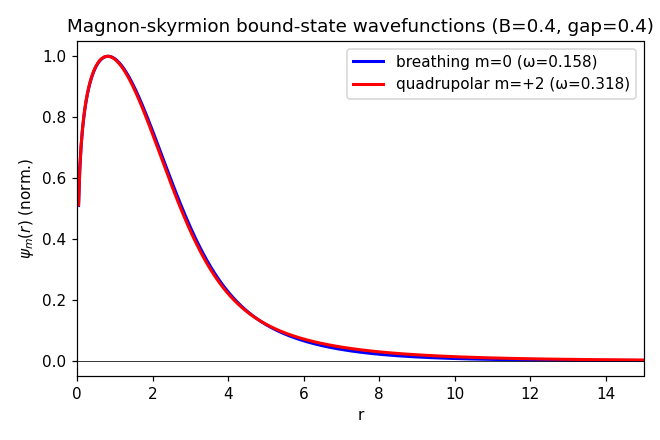
\includegraphics[width=0.6\textwidth]{bound_state_wavefunctions.png}
\caption{Radial wavefunctions of the sub-gap breathing ($m{=}0$) and
quadrupolar ($m{=}\pm2$) bound states.}
\label{fig:wf}
\end{figure}
\begin{figure}[t]
\centering
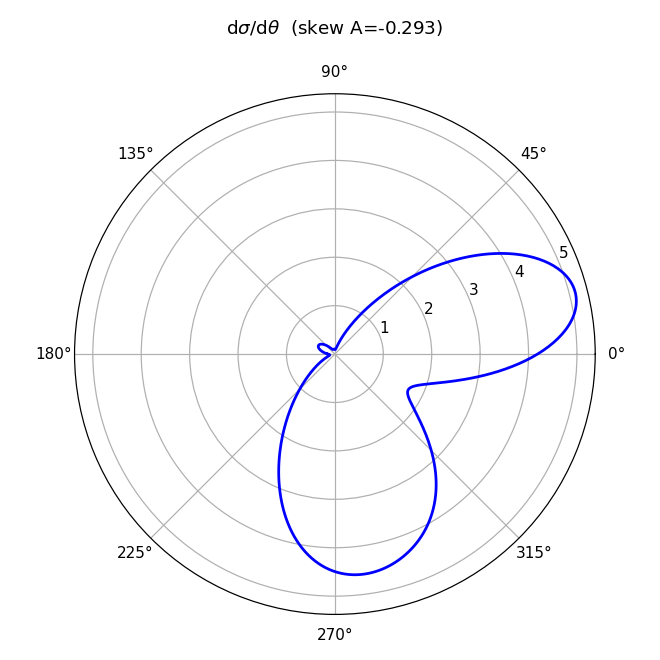
\includegraphics[width=0.48\textwidth]{cross_section_polar.png}
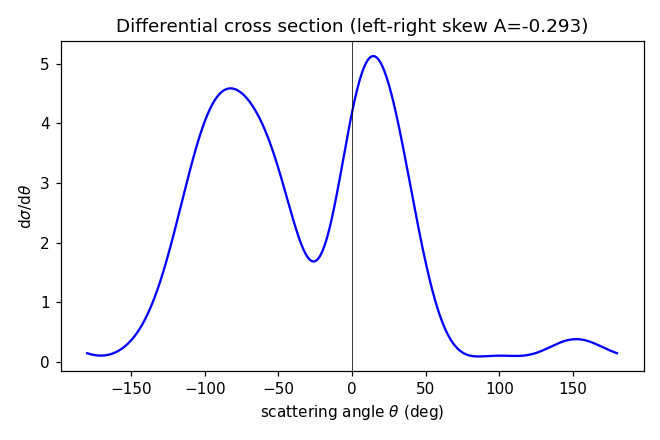
\includegraphics[width=0.48\textwidth]{cross_section_cartesian.png}
\caption{Differential cross section $d\sigma/d\theta$ (polar and cartesian).
The left--right asymmetry ($A=-0.29$) is the skew-scattering signature.}
\label{fig:cs}
\end{figure}

\section{Verdict}
\textbf{PARTIAL$\to$strong (2/2 headline claims reproduced qualitatively).}
Claim~1 (breathing $+$ quadrupolar sub-gap bound states, correct ordering) and
Claim~2 (skew-asymmetric cross section from the emergent flux) are both
reproduced; the stretch Thiele force is confirmed qualitatively. The main
caveats are a single calibration factor $\lambda$ standing in for the full BdG
Hessian (so absolute frequencies, not just structure, would require the
complete second-variation operator) and convention-dependent scattering signs.
See \texttt{failure\_analysis.md} and \texttt{open\_questions.json}.

\end{document}
